% Libro online bastante completo para consulta de Latex: http://en.wikibooks.org/wiki/LaTeX/
% Versión en castellano: http://es.wikibooks.org/wiki/Manual_de_LaTeX
\documentclass[12pt, a4paper, titlepage]{article}

\usepackage[spanish]{babel} % Soporte multilenguaje para LaTeX.

\usepackage[a4paper, top=2.5cm, bottom=2.5cm, left=2.5cm, right=2.5cm]{geometry} % Interfaz flexible para definir las dimensiones del documento

\usepackage[utf8]{inputenc} % Aceptar diferentes tipos de codificación de caracteres de entrada (en este caso usamos la codificación Unicode UTF-8)

\usepackage{graphicx} % Soporte aumentado para gráficos 
\usepackage{hyperref}

\begin{document}

%%%%%%%%%%%%%%%%%%%%%%%%%%%%%%%%%%%%%%%%%%%%%%%%%%%%%%%%%%%%%%%%%%%%%%%%%%%%%%%%
% PORTADA
%%%%%%%%%%%%%%%%%%%%%%%%%%%%%%%%%%%%%%%%%%%%%%%%%%%%%%%%%%%%%%%%%%%%%%%%%%%%%%%%

\begin{titlepage}


\includegraphics[width=15cm]{Imagenes/Simbolo_logo_UDC.png}

% Lista de tamaños: \Huge, \huge, \LARGE, \Large, \large, \small, \footnotesize, \tiny
\vspace{3cm}

\begin{center}

\includegraphics[scale=0.3]{Imagenes/1a_Practica_ER_14-15.png}
\end{center}


\begin{flushright}
	
	\LARGE{\textbf{ JoinMe!}}
	
	\LARGE{\textbf{Modelo del Dominio}}
	
	\large{\textbf{Version 1.0}}
\end{flushright}

\vspace{1cm}
\begin{center}
José Antonio López Sebio\\
Pablo Paz Varela\\
Grupo ER-12-03\\
\end{center}

\vspace{2cm}

\begin{center}
	\large{\textbf{Histórico}}
	
    \begin{tabular}{ | p{4cm} | p{2cm} | p{6cm} | p{3cm} |}
    \hline
    \textbf{Fecha} & \textbf{Version} & \textbf{Descripción} & \textbf{Autor} \\ \hline
      17/03/2014 & 1.0 & Primera Revisión & ER-12-03\\ \hline
      & 1.1 &  & ER-12-03\\ \hline
     &  & &\\ \hline
    \end{tabular}
\end{center}

\end{titlepage}
\clearpage

%%%%%%%%%%%%%%%%%%%%%%%%%%%%%%%%%%%%%%%%%%%%%%%%%%%%%%%%%%%%%%%%%%%%%%%%%%%%%%%%
% INDICE
%%%%%%%%%%%%%%%%%%%%%%%%%%%%%%%%%%%%%%%%%%%%%%%%%%%%%%%%%%%%%%%%%%%%%%%%%%%%%%%%

\tableofcontents
\clearpage

%%%%%%%%%%%%%%%%%%%%%%%%%%%%%%%%%%%%%%%%%%%%%%%%%%%%%%%%%%%%%%%%%%%%%%%%%%%%%%%%
\section{Introducción}
%%%%%%%%%%%%%%%%%%%%%%%%%%%%%%%%%%%%%%%%%%%%%%%%%%%%%%%%%%%%%%%%%%%%%%%%%%%%%%%%
Este documento proporciona el modelado conceptual del dominio de la red social \textbf{joinMe!} , es decir,
muestra clases conceptuales significativas en el dominio del problema.


%%%%%%%%%%%%%%%%%%%%%%%%%%%%%%%%%%%%%%%%%%%%%%%%%%%%%%%%%%%%%%%%%%%%%%%%%%%%%%%%
\section{Modelo del dominio}
%%%%%%%%%%%%%%%%%%%%%%%%%%%%%%%%%%%%%%%%%%%%%%%%%%%%%%%%%%%%%%%%%%%%%%%%%%%%%%%%

En este apartado se describen las clases conceptuales que se extraen de los casos de uso previamente realizados.
\subsection{Usuario}
	Representa al usuario principal de la red social \textbf{joinMe!}, ya que es el usuario que mayor interacción tiene con las funcionalidades del sistema, tales como:
	\begin{itemize}
		\item Agregar amigo.
		\item Comentar publicación.
		\item Gestionar grupo.
		\item Gestionar círculos.
		\item Subir fotografías y vídeos.
		\item etcétera.
	\end{itemize}
	Con esta descripción es obvia la necesidad de modelar al \textbf{Usuario} como una clase conceptual, ya que aparece en la mayoría de los casos de uso. Esta clase tendrá varios atributos, la mayoría de ellos dados por el propio usuario ya que serán sus datos personales.
	Estos atributos son:
	\begin{itemize}
		\item Nombre.
		\item Apellidos.
		\item Teléfono.
		\item Dirección de correo electrónico.
		\item Fotografía de perfil.
	\end{itemize}
	
\subsection{Mensaje}
	Representa un mensaje que es enviado por un usuario a otro usuario contemplada en la funcionalidad de Chat/mensajería. Cada mensaje tiene asociados los siguientes atributos:
	\begin{itemize}
		\item Id.
		\item Fecha y hora de envío.
		\item Texto.
	\end{itemize}
\subsection{Círculo}
	Representa un grupo de Usuarios que son amigos del usuario gestor del círculo. Es decir, es una estructura organizativa de los contactos. Los atributos necesarios en la clase conceptual Círculo son:
	\begin{itemize}
		\item Nombre.
		\item Descripción.
	\end{itemize}
\subsection{Grupo}
	Representa un grupo de Usuarios que se agrupan dentro de la red social, facilitándoles una serie de herramientas para poder discutir o compartir datos referentes a la temática del grupo. Estas funcionalidades pueden ser:
	\begin{itemize}
		\item Muro del grupo.
		\item Foro del grupo.
		\item Compartir fotografías en el grupo.
		\item Compartir videos en el grupo.
	\end{itemize}
	Los atributos que son necesarios para esta clase conceptual son:
	\begin{itemize}
		\item Nombre.
		\item Descripción.
		\item Fecha de creación.
	\end{itemize}
\subsection{Álbum}
	Representa cada álbum donde el usuario organiza las fotografías subidas a la red social \textbf{joinMe!}. Los atributos que contienen la clase conceptual son los siguientes:
	\begin{itemize}
		\item Id.
		\item Nombre
		\item Descripción.
		\item Localización.
		\item Fecha de creación.
		\item Fecha de última modificación.
	\end{itemize}
\subsection{Multimedia}
	Clase conceptual que representa los ficheros de imagen y vídeo que pueden compartir los usuarios de la red social. Contiene los atributos comunes en la red social entre ficheros de imagen y vídeo:
	\begin{itemize}
		\item Id.
		\item Nombre.
		\item Descripción.
	\end{itemize}
\subsection{Fotografía}
	Clase conceptual que representa las fotografías en la red social. Como atributos propios más allá de los heredados de \textbf{Multimedia}, tiene:
	\begin{itemize}
		\item Tamaño.
	\end{itemize}
\subsection{Vídeo}
	Clase conceptual que representa los videos de la red social. Además de los atributos heredados de \textbf{Multimedia}, tiene:
	\begin{itemize}
		\item Duración.
		\item Tamaño.
	\end{itemize}
\subsection{Muro}
	Clase conceptual que representa el muro donde serán publicadas las entradas y las acciones correspondientes a la interacción con las funcionalidades de la red social \textbf{joinMe!} tales como:
	\begin{itemize}
		\item Agregado nuevo contacto.
		\item Fotografía subida.
		\item Vídeo subido.
	\end{itemize}
\subsection{Empresa}
	Clase conceptual que representa al tipo de usuario \textbf{Empresa}, que tiene la posibilidad de crear anuncios para publicitarse en la red social.
\subsection{Anuncio}
	Clase conceptual que representa los anuncios creados por la \textbf{Empresa} y que serán visualizados por los usuarios de la red social. Los atributos necesarios en la clase conceptual Anuncio son:
	\begin{itemize}
		\item Id.
		\item Título.
		\item Fecha de caducidad del anuncio.
	\end{itemize}
\subsection{Categoría}
	Clase conceptual que representa las categorías en las que van clasificadas las entradas de los usuarios así como los anuncios creados por las empresas. Las empresas sólo pueden clasificar sus anuncios en las categorías estándar de la red social, por el contrario los usuarios pueden crear categorías personalizadas.
	Los atributos de esta clase conceptual son:
	\begin{itemize}
		\item Id.
		\item Nombre.
	\end{itemize}
\subsection{Entrada}
	Clase conceptual que representa las entradas creadas por los usuarios o por la red social (nuevas amistades, fotografías subidas...) y que serán publicadas en el Muro, bien en el Muro de cada usuario o bien en el muro de un grupo. 
	Los atributos asociados a esta clase son:
	\begin{itemize}
		\item Id.
		\item Texto.
	\end{itemize}
	Además de los ficheros multimedia que pueda llevar asociados (fotografías y vídeos) y los enlaces.
\subsection{Comentario}
	Representa los comentarios que pueden crear los usuarios y que irán asociados a una publicación, bien sea un fichero multimedia como una fotografía o vídeo, o bien una entrada publicada por un usuario. Los comentarios además del texto podrán contener imágenes y enlaces.
	Los atributos necesarios son:
	\begin{itemize}
		\item Id.
		\item Texto.
	\end{itemize}


%%%%%%%%%%%%%%%%%%%%%%%%%%%%%%%%%%%%%%%%%%%%%%%%%%%%%%%%%%%%%%%%%%%%%%%%%%%%%%%%
\section{Diagrama del Modelo del dominio}
%%%%%%%%%%%%%%%%%%%%%%%%%%%%%%%%%%%%%%%%%%%%%%%%%%%%%%%%%%%%%%%%%%%%%%%%%%%%%%%% 

\begin{center}
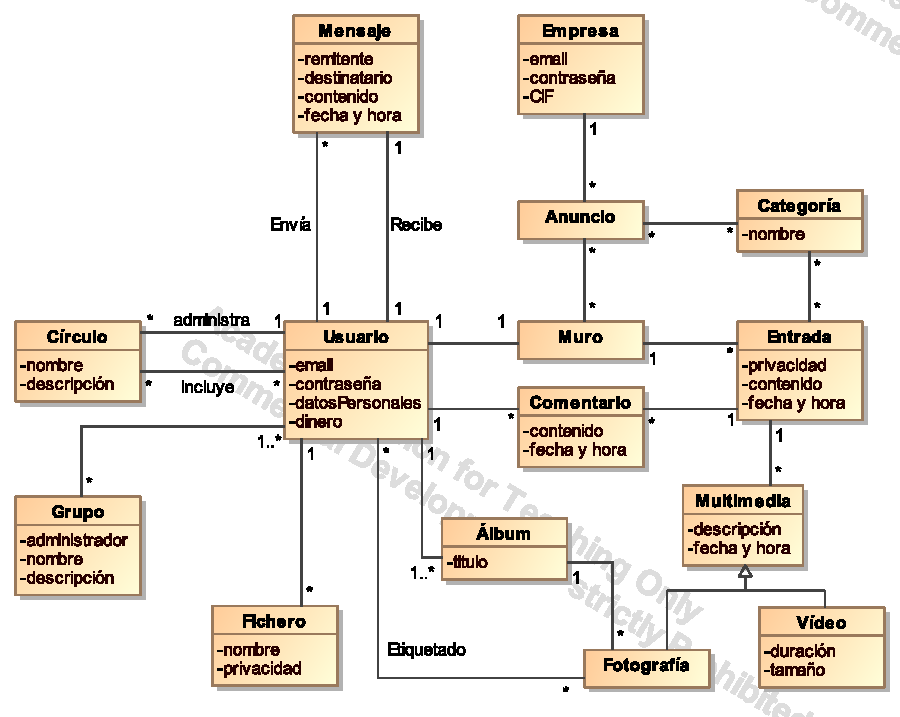
\includegraphics[width=\textwidth]{Imagenes/diagramaModeloDominio}
\end{center}

%%%%%%%%%%%%%%%%%%%%%%%%%%%%%%%%%%%%%%%%%%%%%%%%%%%%%%%%%%%%%%%%%%%%%%%%%%%%%%%% 

\end{document}